\documentclass[letterpaper,10pt,conference]{ieeeconf}
\IEEEoverridecommandlockouts
\overrideIEEEmargins
\usepackage{amsmath,amssymb,booktabs,cite}
\usepackage[T1]{fontenc}
\usepackage{mathptmx,graphicx,microtype,url}
\usepackage[dvipsnames]{xcolor}
\usepackage{tikz}
\usetikzlibrary{arrows.meta,fit,positioning}
\newcommand{\model}{YOLO11-DLA-n}
\title{\LARGE\bf YOLO11-DLA: Fallback-Free Object Detection on NVIDIA DLA\\
for Embedded Robotic Perception}
\author{Anonymous Authors}
\begin{document}
\special{pdf:minorversion 4}
\maketitle
\thispagestyle{empty}
\pagestyle{empty}
\begin{abstract}
Embedded robots share compute resources across perception, localization,
mapping, planning, and control. Dedicated neural accelerators offer additional
placement options, but detector operators and prediction interfaces can
prevent complete learned-graph placement. This work presents YOLO11-DLA, which replaces spatial
self-attention with channel softmax and depthwise convolution, and exports
static multi-scale predictions for host-side decoding and non-maximum suppression.
On Jetson AGX Orin with TensorRT 10.3, the nano model's learned graph compiles into one DLA
loadable without GPU-assigned learned layers in both FP16 and mixed INT8
configurations. On 4,500 COCO validation images excluded from calibration,
strict DLA achieves 37.876 AP in FP16 and 35.408 AP in INT8; the corresponding
adapted GPU engines achieve 37.879 and 35.951 AP. At batch one and
$640\times640$, INT8 reduces strict DLA median engine-plus-transfer latency
from 27.515 to 4.167\,ms and application-pipeline latency from 56.820 to
30.675\,ms. Module energy at 10\,Hz decreases from 0.874 to 0.806\,J/frame.
The adapted INT8 GPU engine remains faster and lower-energy, at 18.212\,ms
application-pipeline latency and 0.760\,J/frame. The contribution combines verified
learned-graph placement with application-level characterization of
precision-dependent accuracy, latency, host-side processing, and energy
trade-offs for embedded robotic perception, rather than universal accelerator
superiority.
\end{abstract}
\section{Introduction}
\label{sec:introduction}
Embedded robots combine perception, localization, mapping, planning, and
control on shared compute resources. Heterogeneous platforms provide CPUs,
GPUs, and dedicated neural accelerators, but assigning a workload to an
auxiliary accelerator requires knowing which computation resides there.
A detector intended for the NVIDIA Deep Learning Accelerator (DLA) may still
use GPU kernels.

This work distinguishes nominal DLA deployment from verified fallback-free placement
of the learned graph. TensorRT can request DLA execution while permitting
unsupported regions to fall back to GPU \cite{nvidia_dla_working}. Operator
support, tensor shapes, normalization axes, precision, and I/O layouts constrain
placement. GPU efficiency and successful export do not certify complete
execution on a restricted accelerator.

YOLO11 \cite{jocher2024yolo11} is a representative case: its convolutional
backbone and neck coexist with spatial self-attention and a decoded prediction
interface. Attention matrix products and the flattened prediction path obstruct
strict DLA compilation in the tested configuration. The study examines how
localized architectural and interface changes enable complete learned-graph
placement,
and what accuracy, latency, host-side processing, and energy costs follow.

\begin{figure}[t]
    \centering
    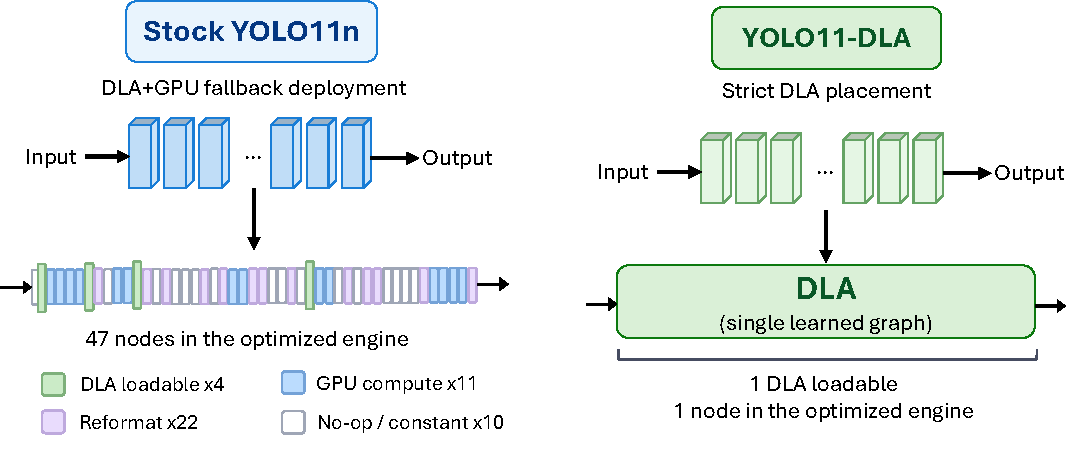
\includegraphics[width=\columnwidth]{figures/teaser.pdf}
    \caption{FP16 deployment. Stock YOLO11n uses DLA+GPU fallback;
    YOLO11-DLA places the complete learned graph in one DLA loadable.
    Host-side decoding and non-maximum suppression remain outside the accelerator.}
    \label{fig:teaser}
\end{figure}

YOLO11-DLA combines architectural adaptation and a static export boundary
for verified placement (Fig.~\ref{fig:teaser}). C2DLA replaces incompatible
spatial attention with channel mixing and local convolution; three raw static
prediction maps define the output boundary. Host-side decoding, confidence
filtering, and non-maximum suppression (NMS) execute on the host. The nano
instance is denoted \model. Recovering GPU capacity for another robotic
workload remains a system-level hypothesis.

This work develops a hardware/software co-design approach for verified
learned-graph placement. First, an architectural adaptation removes accelerator-incompatible
learned computation, and an explicit static prediction boundary separates the
remaining learned graph from host-side decoding and variable-cardinality
post-processing, retaining YOLO11's surrounding architecture and training
formulation. Second, fallback-disabled compilation
and optimized-engine inspection verify placement, while native I/O handling
connects the DLA loadable to the host runtime. Third, deployed-engine evaluation
measures accuracy, engine-plus-transfer latency, application-pipeline latency,
host-side overhead, and module energy at a matched delivered rate in FP16
and calibrated INT8, with GPU controls for both models.
The engine-plus-transfer latency advantage over stock fallback reverses in
application-pipeline latency, demonstrating why placement must be assessed
jointly with accuracy, host-side overhead, and the operating point.

\section{Related Work}
\label{sec:related}
\paragraph*{Efficient object detection}

YOLO evolved from single-network detection \cite{redmon2016yolo} through
multi-scale prediction and feature/training refinements
\cite{redmon2018yolov3,bochkovskiy2020yolov4}, anchor-free heads and assignment
\cite{ge2021yolox}, deployment-oriented structures \cite{li2022yolov6},
training and aggregation improvements \cite{wang2023yolov7,wang2024yolov9},
and NMS-free prediction \cite{wang2024yolov10}. These developments motivate
YOLO11 as a representative detector; GPU benchmarking does not establish
complete placement on DLA. YOLO11's detection towers and distributional
regression are retained \cite{jocher2024yolo11,li2020gfl}. Its surrounding
structure draws on feature partitioning and pyramid aggregation
\cite{wang2020cspnet,lin2017fpn,liu2018panet}. Unlike RepVGG-style deployment
re-parameterization \cite{ding2021repvgg,li2022yolov6}, the proposed adaptation changes
the incompatible attention computation while preserving this surrounding
structure. The objective is accelerator-compatible deployment rather than
optimization of the AP/FLOPs trade-off.

\paragraph*{Hardware-aware and edge network design}

YOLO-ReT and YOLOBench address edge-GPU detection and controlled evaluation
across embedded hardware \cite{ganesh2022yoloret,lazarevich2023yolobench}.
ActNAS examines hardware-sensitive activation choices, including compiler
effects \cite{sah2025actnas}. MnasNet and ProxylessNAS incorporate target
latency into architecture selection \cite{tan2019mnasnet,cai2019proxyless};
Once-for-All supports deployment specialization \cite{cai2020ofa}; MCUNet
co-designs networks and runtime \cite{lin2020mcunet}. Here strict compilation
is a feasibility constraint for a manually specified adaptation. C2DLA uses
projection and normalization related to external attention
\cite{guo2023external}, but only mixes channels at each position and adds
local depthwise context. It does not reproduce full external attention or
claim representational superiority.

\paragraph*{Heterogeneous accelerator deployment for embedded perception}
Archet et al.\ \cite{archet2023energy} study CNN design and inference options
on Jetson AGX Orin, showing that its CPU, GPU, and DLA offer different latency
and energy trade-offs. Hern\'andez et al.\ \cite{hernandez2024optimizing}
evaluate quantization on AGX Orin and report that DLA layer incompatibilities
degrade inference performance and efficiency in their tested models.
These studies make network compatibility part of the practical
accelerator-selection problem.

Tayal and Simmhan \cite{tayal2024multiinstance} examine multi-instance inference
across Orin's CUDA cores, Tensor Cores, and DLAs, investigating resource
congestion under concurrent workloads. Chakraborty et al.\
\cite{chakraborty2025profiling} profile concurrent vision inference on Jetson,
linking throughput degradation to resource contention and CPU--GPU scheduling;
aggregate GPU utilization alone does not describe component-level efficiency.
These findings motivate explicit workload placement, without establishing
concurrent-task benefits for the adapted detector.

Compiler lowering \cite{chen2018tvm} and TensorRT's optional GPU fallback
\cite{nvidia_dla_working} make compatibility an architectural and deployment
property, not merely an exporter setting. The proposed architectural adaptation
and static prediction boundary support fallback-disabled compilation and
optimized-engine placement verification, evaluated separately from deployed
accuracy, latency, host-side overhead, and module energy.

\section{YOLO11-DLA}
\label{sec:method}
\begin{figure*}[t]
\centering
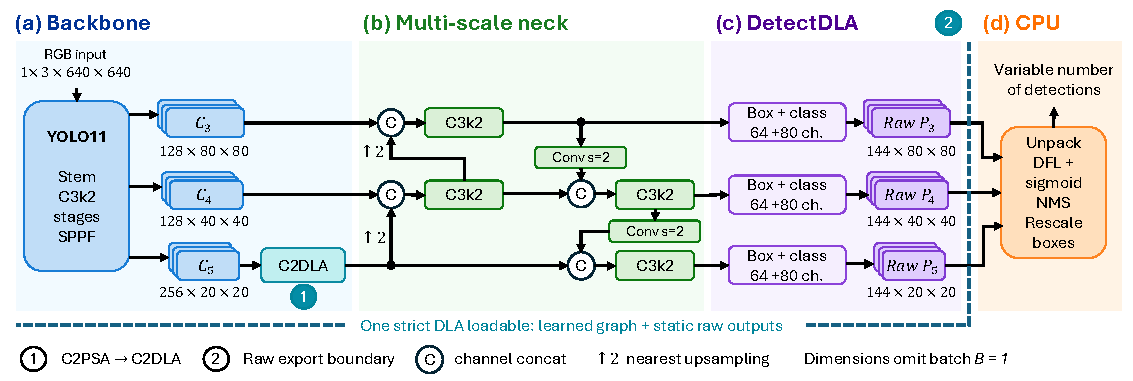
\includegraphics[width=0.95\textwidth]{figures/architecture_overview.pdf}
\caption{\textbf{YOLO11-DLA architecture.} Backbone scales feed the neck and box/class
 towers at strides 8, 16, and 32. Markers 1 and 2 identify C2DLA and the raw-output
 boundary. The learned graph forms one DLA loadable; unpacking and post-processing
 remain on CPU. Preprocessing and input packing precede the graph.}
\label{fig:boundary}
\end{figure*}

\subsection{Design Objective and Scope}
This work treats learned-graph placement as a design constraint for embedded
robotic perception. Let $G$ denote the learned graph obtained by adapting the
reference YOLO11 graph. The design goal is to obtain a useful detector whose
complete learned computation can be assigned to the tested DLA configuration:
\begin{equation}
 \operatorname{Build}_{\mathrm{DLA}}(G;\theta,\mathrm{fallback}=0)
 = E, \qquad N_{\mathrm{GPU}}(E)=0,
 \label{eq:accept}
\end{equation}
where $\theta$ fixes the target, compiler version, precision, shapes, and
I/O formats, $E$ is the serialized engine, and $N_{\mathrm{GPU}}$ counts
GPU-assigned learned layers after optimization. For each evaluated strict
engine, one DLA loadable is also required. These are deployment criteria, not training-loss
terms; accuracy and application performance are evaluated after this gate.

The convolutional stem, C3k2 stages, SPPF module, feature-pyramid connections,
and detection towers of YOLO11n are retained (Fig.~\ref{fig:boundary}). Two module substitutions define
the adaptation:
\begin{equation}
 \mathrm{C2PSA}\longrightarrow\mathrm{C2DLA},\qquad
 \mathrm{Detect}\longrightarrow\mathrm{DetectDLA}.
 \label{eq:substitutions}
\end{equation}
The first substitution changes an accelerator-incompatible learned computation;
the second defines a static accelerator boundary while preserving the ordinary
training path. Together they retain the surrounding YOLO11 backbone, neck,
and detection towers. The adapted GPU engine provides a same-model placement
control; comparisons with stock YOLO11n additionally include architectural and
training differences and use different prediction interfaces.

\subsection{C2DLA: Channel Mixing with Local Context}
\label{sec:c2dla}
\begin{figure*}[t]
\centering
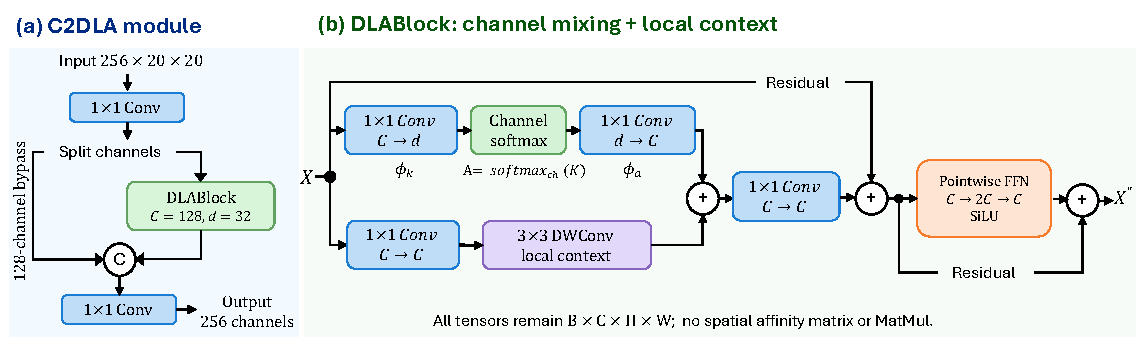
\includegraphics[width=0.90\textwidth]{figures/c2dla_detail.pdf}
\caption{\textbf{C2DLA module and operators.} (a) Nano-model split--process--merge block
 at $20\times20$. (b) Channel softmax and local depthwise convolution replace spatial
 attention, retaining both residual additions and the pointwise FFN.
 C denotes concatenation; $+$ denotes elementwise addition.}
\label{fig:c2dla}
\end{figure*}

C2DLA keeps C2PSA's split--process--merge structure (Fig.~\ref{fig:c2dla}). An initial $1\times1$
projection produces two channel groups; one bypasses the inner block and the
other is processed before concatenation and a final projection. If $X$ is the
processed group with $C$ channels, define
\begin{align}
 K &= \phi_k(X), \qquad V=\phi_v(X), \label{eq:kv}\\
 A_{bkhw} &= \frac{\exp K_{bkhw}}{\sum_{j=1}^{d}\exp K_{bjhw}},
 \label{eq:chansoftmax}\\
 Z &= \phi_o\bigl(\phi_a(A)+\psi_{3\times3}(V)\bigr),
 \label{eq:mix}\\
 X' &= X+Z, \label{eq:res1}\\
 X'' &= X'+\operatorname{FFN}(X'). \label{eq:res2}
\end{align}
Here $d=\max(\lfloor C/4\rfloor,8)$; $\phi_k:C\to d$,
$\phi_v:C\to C$, $\phi_a:d\to C$, and $\phi_o:C\to C$ are
$1\times1$ projections. The operator $\psi$ is a $3\times3$ depthwise
convolution. The FFN expands channels from $C$ to $2C$, applies SiLU, and
projects back to $C$. Batch normalization accompanies the relevant convolution
modules and is folded into them for inference; $\phi_a$ is a bias-free
convolution without batch normalization.

For the nano configuration, the enclosing block receives 256 channels, the
processed group has $C=128$, the bottleneck has $d=32$, and one inner block
operates at the $20\times20$ scale. All operations preserve the four-dimensional
batch--channel--height--width representation. Unlike the original attention,
there is no spatial affinity matrix, matrix multiplication, head transpose,
or normalization over image positions.

This hardware-aware substitute uses input-dependent channel mixing and
local depthwise context while operating on static four-dimensional tensors and
avoiding spatial affinity matrices and MatMul. It does not exchange information
between distant positions. The substitution changes the hypothesis class and
requires empirical accuracy evaluation; it is not algebraically equivalent to
C2PSA, nor is greater representational power claimed.

The key and value projections are separate convolutions. This avoids introducing
a fused-QKV extraction subgraph in the replacement branch. Static channel
splits elsewhere in the retained graph remain present and compile successfully
in the measured configuration. Thus, the implementation does not depend on a
claim that every split or SiLU is unsupported on DLA.

\subsection{DetectDLA: A Static Prediction Boundary}
\label{sec:boundary}
For each pyramid level $\ell\in\{3,4,5\}$, the retained regression and
classification towers produce $R_\ell$ and $S_\ell$. DetectDLA exports
\begin{equation}
 P_\ell=\operatorname{Concat}_{C}(R_\ell,S_\ell)
 \in\mathbb{R}^{B\times(4r+n_c)\times H_\ell\times W_\ell},
 \label{eq:packed}
\end{equation}
with $r=16$ regression bins and $n_c=80$ COCO classes. For batch one and
$640\times640$ images, the outputs are $1\times144\times80\times80$,
$1\times144\times40\times40$, and $1\times144\times20\times20$ at strides
8, 16, and 32. They are named \texttt{pred\_p3}, \texttt{pred\_p4}, and
\texttt{pred\_p5}. Classification values are logits; box channels are
unnormalized distributions, not decoded coordinates.

DetectDLA defines the boundary between a static learned accelerator graph and
host-side detection processing. Export stops before flattening, cross-scale
concatenation, the expectation over the DFL regression distribution, grid
decoding, and
sigmoid; confidence filtering and variable-cardinality NMS remain outside the
engine. During training and ordinary PyTorch inference, DetectDLA invokes the
inherited Detect path, retaining its losses and assignment behavior. The change
concerns deployment partitioning, not a direct-regression or one-to-one
prediction formulation.

The static maps make the execution boundary explicit. Stock YOLO11n's engine
instead emits a decoded $1\times84\times8400$ tensor. At FP16, the adapted
outputs contain 2,419,200 bytes, compared with 1,411,200 bytes for the stock
output, a factor of 1.714. Consequently, lower engine-plus-transfer latency does
not by itself establish a faster end-to-end detector pipeline: the adapted FP16
pipeline transfers more data and performs decoding on the host.


\subsection{Training and Initialization}
The nano model is initialized from pretrained YOLO11n weights. The loader
intersects the source and destination state dictionaries by tensor name and
shape, copies compatible entries, and loads them non-strictly. Unmatched
parameters retain their model initialization. This transfers the compatible
backbone, neck, detection towers, and matching parts of the replacement block
without requiring a correspondence between spatial attention and channel mixing.
All trainable layers are subsequently fine-tuned; the procedure does not
require a separate frozen-backbone stage or a specialized QKV remapping.

The model is fine-tuned on COCO train2017 for 500 epochs, with batch size 32,
$640\times640$ images, seed 0, automatic mixed precision (AMP), and no
user-frozen layers. The model contains 2,615,696 unfused parameters. In the
training implementation used for these experiments,
\texttt{optimizer=auto} selects MuSGD for this training budget, with base
learning rate 0.01, momentum 0.9, and weight decay $5\times10^{-4}$.
The schedule has three warm-up epochs followed by linear decay to 0.01 of
the base learning rate; selected classification-head parameter groups use
a threefold learning-rate multiplier. The recorded group learning rates
are consistent with this configuration.

Training uses HSV perturbation, translation, scaling, horizontal flips, and
mosaic augmentation; mosaic is disabled for the final ten epochs. MixUp and
copy-paste are disabled. These settings describe fine-tuning of the adapted
model from stock weights, not equal-budget retraining of both architectures, so
the comparison evaluates the resulting detectors rather than the substitution
alone.

\section{Export and Runtime}
\label{sec:deployment}
\subsection{Exported Graph and Strict Compilation}
The exported ONNX graph uses opset 20 and a static $1\times3\times640\times640$
input. Inspection finds 89 convolutions, 76 sigmoid and 76 multiplication nodes,
9 splits, 14 additions, 20 concatenations, 3 max-pooling operations, 2 resizes,
and one softmax. There are no MatMul, Gemm, Reshape, Transpose, Div, or Slice
operators. The sigmoid/multiplication pairs represent retained SiLU activations;
operator counts before fusion are not execution-kernel counts.

Compilation targets DLA core 0 in FP16 and calibrated INT8 with GPU fallback
disabled and explicit native I/O formats. Successful compilation is checked against both the verbose
placement report and the optimized-engine inspector. For each strict optimized engine,
the inspector reports a single DLA node corresponding to one DLA loadable; this
does not mean that the source graph contains one operation. Build and profile
records identify engine name, compiler version, and output bindings.

This placement verification is configuration-specific. TensorRT's DLA softmax support depends on
the target and shape, and the compiler warns that the selected approximation
can introduce numerical error \cite{nvidia_dla_working}. A source-level
rewrite that compiles on this Orin/TensorRT combination is not sufficient
evidence for another DLA generation, input size, or precision. Build success
also does not validate raw-output decoding.

\subsection{Native Layouts and the Host Boundary}
\label{sec:packing}
The FP16 strict build requests \texttt{fp16:dla\_hwc4} input and
\texttt{fp16:chw16} outputs. The input pads three channels to four in
interleaved storage, occupying $4\times640\times640\times2=3{,}276{,}800$
bytes. Output channels (144) are divisible by 16, requiring no channel padding.
The INT8 strict engine instead uses \texttt{int8:dla\_hwc4} input and
\texttt{int8:chw32} outputs. Its input occupies 1,638,400 bytes; CHW32 pads
144 channels to 160, totaling 1,344,000 output bytes across the three levels.
Both input layouts satisfy the documented row alignment
\cite{nvidia_dla_working}. GPU and stock DLA+GPU fallback engines retain linear FP16
external bindings in both precision modes.

For native INT8 bindings, the host quantizes normalized pixels as
$q=\operatorname{clip}(\operatorname{round}(x/s),-128,127)$ and dequantizes
raw outputs as $y=sq$. Per-tensor scales are read from the model's calibration
cache and checked against the explicit build-time I/O ranges; engine-hash-bound
metadata supplies the runtime scales. Thus, changing precision changes both
arithmetic and the host I/O path, not just the serialized engine.

The reference runner performs packing, unpacking, and INT8 conversion on the
CPU. Timed input stages include packing and host-to-device (H2D) transfer;
output stages include device-to-host (D2H) transfer, unpacking, and any
dequantization. These are not pure layout-conversion timings. A CUDA stream
and device-visible buffers remain necessary without GPU-assigned learned layers.
Logical shape alone is insufficient, so formats, vectorized dimensions,
component counts, and context strides are recorded. For the FP16 engine,
TensorRT reports CHW4 input and CHW16 outputs; the padded input interpretation
is validated for this shape, not for arbitrary CHW4 bindings.

\subsection{Confidence-First Host Decoding}
\label{sec:decode}
The host splits each $P_\ell$ into 64 regression channels and 80 class channels.
For confidence threshold $\tau\in(0,1)$, an anchor survives if
\begin{equation}
 \sigma\!\left(\max_c S_{\ell,c}(h,w)\right) > \tau.
 \label{eq:threshold}
\end{equation}
The implementation applies sigmoid before the comparison to preserve dense
floating-point threshold behavior. Regression decoding is independent of
class confidence and is postponed until after rejection. For each
survivor and box side $q\in\{l,t,r,b\}$, the DFL expectation is
\begin{equation}
 \hat d_q=\sum_{j=0}^{r-1}j\,
 \frac{\exp R_{qj}}{\sum_{k=0}^{r-1}\exp R_{qk}}.
 \label{eq:dfl}
\end{equation}
The decoder places cell centers at $(w+0.5,h+0.5)$, forms the four box
coordinates from these distances, scales by the level stride, applies class
sigmoid, and performs class-aware NMS. The final coordinates are mapped back
through the image's letterbox transform.

If $m$ of $N=8400$ anchors survive, dense class scanning remains
$O(Nn_c)$, while the regression softmax/expectation work falls from $O(4rN)$
to $O(4rm)$. This does not reduce raw-output transfer volume. In the FP16 strict
10\,Hz test, surviving anchors range from 0 to 254, with median 28.5 over the
100-image cycle. Identical threshold strictness, class selection, NMS settings,
and tie handling are necessary for dense/sparse agreement.

\section{Experimental Evaluation}
\label{sec:eval}
The evaluation considers fallback-free placement, deployed accuracy,
engine-plus-transfer latency, application-pipeline latency, and module energy
at a matched delivered
rate; engine hashes, per-image predictions, timing records, and power traces
connect the compiled configurations to measured behavior. Each precision mode
includes stock YOLO11n on GPU and with DLA+GPU fallback (stock fallback), and \model\ on GPU
and strict DLA. Tables abbreviate these models as 11n and 11-DLA; DLA denotes
strict placement for the adapted model.

\subsection{Platform and Precision Protocol}
\label{sec:setup}
Tests use an NVIDIA Jetson AGX Orin Developer Kit with L4T 36.4.4, CUDA runtime
12.6, TensorRT 10.3.0, PyTorch 2.5.0a0, and ROS~2 Jazzy. The platform is
configured in NVIDIA's 50\,W power mode with \texttt{jetson\_clocks} disabled;
CPU frequencies vary during measurement. Strict execution targets DLA core 0,
and the benchmark is a standalone runner rather than a ROS~2 node.
All configurations use batch one and $640\times640$ inputs. FP16 enables
half precision; INT8 enables both INT8 and FP16. These names describe build
modes, not uniform precision of every operation: GPU regions may retain
FP16/FP32 intermediates.

Post-training calibration uses 500 COCO val2017 images sampled without
replacement with seed 2027, leaving 4,500 disjoint images for accuracy
\cite{lin2014coco}. The two ONNX models have separate entropy-calibration
caches, generated before fusion with TensorRT's EntropyCalibrator2 using the
same image IDs, batch one, and normalized FP32 RGB letterboxed inputs.
No labels enter calibration, and INT8 entails no additional training. Each
model's cache is shared across its GPU and DLA placements. The calibrated
engines and native I/O scales are validated before evaluation.

\subsection{Fallback-Free Placement}
\label{sec:placement}
Stock YOLO11n fails strict FP16 compilation at its attention MatMul; no
fallback-disabled stock INT8 build was attempted. The
adapted FP16 build assigns 299 layers to DLA and none to GPU. Both adapted
strict engines have one optimized DLA node corresponding to one loadable,
with no GPU or reformat nodes. The INT8 build assigns 298 layers to INT8 and
one softmax to FP16, all on DLA. Fallback-disabled compilation and inspection
therefore satisfy Eq.~\eqref{eq:accept} for both tested precision modes;
fallback-free does not imply integer-only computation.

The stock FP16 fallback engine instead contains four DLA loadables, eleven GPU
compute nodes, twenty-two reformats, and ten no-op/constant nodes. Its separate
layer profile attributes 93.97\% of time to DLA, 4.73\% to reformats, and
1.30\% to GPU computation (Fig.~\ref{fig:profile}); the summed device profile
is 34.312\,ms, including 32.244\,ms in DLA segments. Stock INT8 fallback also
has four DLA loadables, with twenty-three reformats among 48 optimized nodes.
Comparing these heterogeneous deployments with strict DLA includes changed
attention and output boundaries and does not isolate partitioning cost.

\begin{figure}[t]
\centering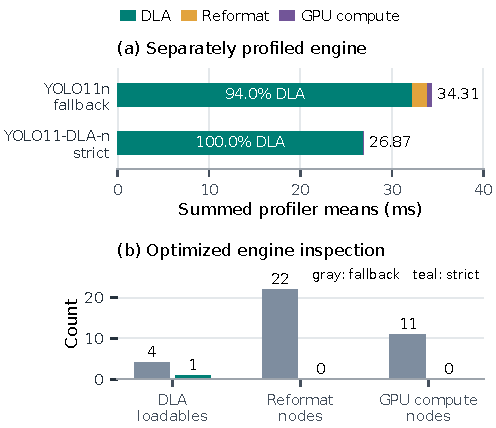
\includegraphics[width=\columnwidth]{figures/fallback_profile.pdf}
\caption{FP16 placement and separate layer profiles. Stock fallback has four
DLA loadables and intervening GPU/reformat work; the adapted strict engine has
one DLA loadable. These time shares characterize FP16, not INT8.}
\label{fig:profile}
\end{figure}

\subsection{Engine-Plus-Transfer Latency and Throughput}
\label{sec:engine}
The \texttt{trtexec} microbenchmark uses a 2\,s warm-up, a 30\,s timing window,
one inference stream, spin waiting, generated input data, and transfers enabled:
\begin{equation}
 L_{\mathrm{engine+IO}}=T_{\mathrm{H2D}}+T_{\mathrm{device}}+T_{\mathrm{D2H}}.
 \label{eq:latency}
\end{equation}
This boundary excludes preprocessing, host-side decoding, and NMS. TensorRT's
``GPU Compute Time'' field measures device execution even for a DLA engine;
it does not establish GPU computation. Query throughput uses host wall time
and can differ from reciprocal median latency because transfers and execution
overlap. Profiles are collected separately. P95 and P99 characterize frame
variation within tests, not confidence intervals across independent trials.

\begin{table}[t]
\caption{Engine-plus-transfer latency, batch one, $640\times640$. Median and P95 are milliseconds; rate is queries/s.}
\label{tab:engine}\centering\footnotesize
\setlength{\tabcolsep}{3pt}
\begin{tabular*}{\columnwidth}{@{\extracolsep{\fill}}llrrr@{}}
\toprule
Model / device & Mode & Median & P95 & Rate \\
\midrule
11n / GPU & FP16 & 3.740 & 3.753 & 288.3 \\
11n / DLA+GPU & FP16 & 34.678 & 34.942 & 29.2 \\
11-DLA / GPU & FP16 & 3.500 & 3.512 & 317.2 \\
11-DLA / DLA & FP16 & 27.515 & 27.718 & 37.2 \\
\midrule
11n / GPU & INT8 & 3.021 & 3.030 & 357.0 \\
11n / DLA+GPU & INT8 & 13.068 & 13.094 & 79.5 \\
11-DLA / GPU & INT8 & 2.828 & 2.836 & 393.4 \\
11-DLA / DLA & INT8 & 4.167 & 4.173 & 263.7 \\
\bottomrule
\end{tabular*}
\end{table}

\begin{figure}[t]
\centering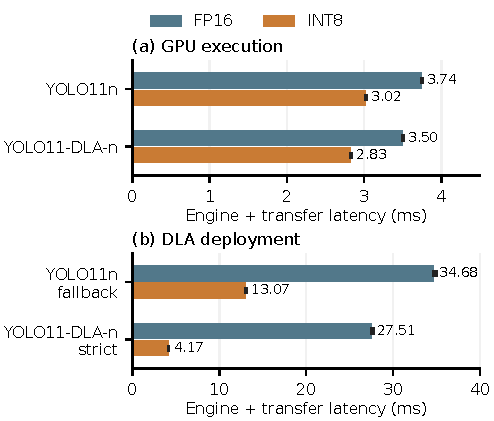
\includegraphics[width=\columnwidth]{figures/precision_latency.pdf}
\caption{FP16 and INT8 engine-plus-transfer latency. Bars show medians and
whiskers extend to P95; panels use different horizontal scales. INT8 provides
a larger relative reduction for strict DLA than for the GPU controls.}
\label{fig:latency}
\end{figure}

Table~\ref{tab:engine} and Fig.~\ref{fig:latency} show that INT8 reduces strict DLA
median engine-plus-transfer latency from 27.515 to 4.167\,ms, a $6.60\times$ speedup, and increases
throughput from 37.2 to 263.7 queries/s. Strict DLA has lower
engine-plus-transfer latency than stock fallback in both modes: 20.7\% lower
median in FP16 and a $3.14\times$ reduction in INT8. The same adapted model on
GPU remains faster at this boundary: 3.500\,ms in FP16 and 2.828\,ms in INT8. Strict INT8 device execution alone
is 3.789\,ms. Neither result establishes comparable accuracy or application
performance.

\subsection{Deployed-Engine Accuracy}
\label{sec:accuracy}
The main comparison evaluates all eight configurations on the same 4,500
held-out IDs, verifying matching image hashes. FP16 predictions from the
existing 5,000-image evaluation are rescored on this subset without rerunning
inference. Preprocessing centers a square $640\times640$ letterbox with padding
114 and RGB normalization by 255. CPU post-processing uses confidence 0.001,
class-aware NMS at intersection over union (IoU) 0.7, multi-label candidates,
and at most 300 boxes per image; COCOeval uses standard detection limits.
These settings differ from the timing thresholds.

\begin{table}[t]
\caption{Accuracy on 4,500 held-out COCO val2017 images, disjoint from INT8 calibration. AP values are percentage points; INT8 allows mixed precision; stock and adapted training budgets differ.}
\label{tab:accuracy}\centering\footnotesize
\setlength{\tabcolsep}{3pt}
\begin{tabular*}{\columnwidth}{@{\extracolsep{\fill}}llrrr@{}}
\toprule
Model / device & Mode & AP & AP$_{50}$ & AP$_{75}$ \\
\midrule
11n / GPU & FP16 & 39.378 & 55.190 & 42.845 \\
11n / DLA+GPU & FP16 & 39.308 & 55.160 & 42.823 \\
11-DLA / GPU & FP16 & 37.879 & 53.633 & 41.008 \\
11-DLA / DLA & FP16 & 37.876 & 53.614 & 41.016 \\
\midrule
11n / GPU & INT8 & 33.175 & 47.324 & 36.069 \\
11n / DLA+GPU & INT8 & 19.827 & 35.241 & 20.867 \\
11-DLA / GPU & INT8 & 35.951 & 51.063 & 39.323 \\
11-DLA / DLA & INT8 & 35.408 & 50.790 & 38.614 \\
\bottomrule
\end{tabular*}
\end{table}

Table~\ref{tab:accuracy} separates precision loss from placement effects.
Strict INT8 loses 2.468 AP points relative to strict FP16; adapted GPU loses
1.928 points. Within a precision mode, strict DLA minus adapted GPU AP is
$-0.003$ points in FP16 and $-0.543$ in INT8. Thus, the negligible FP16
placement difference does not extend unchanged to INT8.
Stock GPU loses 6.203 points, while stock fallback loses 19.48 AP points,
reaching only 19.827 AP. Under this calibration protocol the adapted INT8
engines exceed stock INT8 accuracy, but the fallback result is not an
accuracy-equivalent baseline: its degradation has no isolated causal
explanation here, and architecture, training, and calibration differences
preclude a general claim about quantization robustness.

The original full-5,000-image FP16 AP values are 39.314 (stock GPU), 39.245
(stock fallback), 37.995 (adapted GPU), and 37.991 (strict DLA); they must not
be compared directly with held-out INT8 AP.
The adapted checkpoint's stored 500-epoch validation history ends at AP 37.581
and AP$_{50}$ 53.151 under a different evaluation protocol; these training
metrics do not establish an export-induced gain.

\subsection{Export, Layout, and Decoder Checks}
\label{sec:parity}
A CPU check on one random input (seed 7) finds maximum external-decoder error
$1.22\times10^{-4}$ and raw-map ONNX/checkpoint error $3.07\times10^{-4}$;
these are distinct from engine validation. On 50 real images, each
precision campaign passes eight layout checks and 200 dense/sparse decoder
comparisons: two engines and two confidence settings (0.001 multi-label and
0.25 single-label). The exploratory raw GPU/DLA comparison, at absolute
and relative tolerances 0.1 and 0.05, fails on 50/49/49 images for FP16
P3/P4/P5 and on all 50 at every level for INT8. Raw agreement is therefore
reported diagnostically, not claimed as a passed numerical gate.

On all 5,000 images, FP16 dense/sparse AP differs by less than $10^{-7}$
points; one GPU image (74092) has 252 sparse versus 251 dense detections.
On the 4,500 held-out images, INT8 dense/sparse AP is identical at reported
precision for both adapted engines, but GPU image 408774 has 295 sparse
versus 294 dense detections. Aggregate accuracy agreement does not establish
bitwise identity or equality of every post-NMS detection.

\subsection{Multi-Image Application Pipeline}
\label{sec:application}
The sequential runtime preloads the same first 100 validation images in sorted
ID order for both precisions, then cycles through them for 60\,s after 30
warm-up frames and 30\,s stabilization. CPU preprocessing and NMS use one
thread, confidence 0.25, single-label candidates, and NMS IoU 0.45; adapted
engines use sparse decoding.
The boundary includes native I/O and any quantization/dequantization, and
excludes disk access, visualization, camera acquisition, and ROS transport.
Faster configurations complete more cycles within the fixed duration.

\begin{table*}[t]
\caption{Application pipeline on the same 100 images, 60\,s per test. Latency: ms; rate: frames/s. Includes preprocessing, native I/O, inference, decode and NMS.}
\label{tab:e2e}\centering\footnotesize
\setlength{\tabcolsep}{4pt}
\begin{tabular*}{\textwidth}{@{\extracolsep{\fill}}lrrrrrrrr@{}}
\toprule
& \multicolumn{4}{c}{FP16} & \multicolumn{4}{c}{INT8} \\
\cmidrule(lr){2-5}\cmidrule(l){6-9}
Model / device & Median & P95 & P99 & Rate & Median & P95 & P99 & Rate \\
\midrule
11n / GPU & 20.030 & 24.658 & 27.702 & 47.99 & 17.556 & 22.104 & 23.681 & 54.70 \\
11n / DLA+GPU & 51.241 & 59.542 & 64.478 & 18.95 & 29.020 & 37.510 & 40.293 & 32.71 \\
11-DLA / GPU & 20.307 & 24.584 & 28.591 & 47.63 & 18.212 & 22.467 & 23.780 & 53.00 \\
11-DLA / DLA & 56.820 & 65.042 & 76.886 & 17.19 & 30.675 & 34.812 & 36.322 & 31.93 \\
\bottomrule
\end{tabular*}
\end{table*}

INT8 reduces strict DLA median application-pipeline latency from 56.820 to 30.675\,ms,
a $1.85\times$ speedup (Table~\ref{tab:e2e}). This is substantially smaller
than the engine speedup. Strict INT8 input packing/quantization/H2D has median
7.463\,ms, inference 4.522\,ms, output transfer/unpacking/dequantization
10.729\,ms, and post-processing 4.628\,ms. Stock INT8 fallback has corresponding
medians 2.318, 13.467, 1.500, and 5.830\,ms. Native I/O processing thus remains
a substantial cost in this implementation. Stage medians do not sum to median
total latency, and the inference stage includes runtime-call and synchronization
overhead beyond device execution.

The engine ordering reverses at the application boundary in both modes:
strict latency exceeds fallback by 10.9\% in FP16 and 5.7\% in INT8. Adapted
INT8 GPU is faster still, at 18.212\,ms. Host effects also vary: INT8 median
preprocessing is 2.954\,ms for strict DLA versus 5.568\,ms for fallback on
the same images. These tests characterize the observed runtime rather than
isolating hardware costs.

\subsection{Module Energy at a Matched Delivered Rate}
\label{sec:energy}
Energy tests schedule the same 100-image cycle at 10\,Hz for 60\,s, with the
application thresholds and warm-up/stabilization protocol above. Every active
configuration completes 600 frames, six per image, without observed drops or
misses of the 100\,ms release-to-result deadline.

\texttt{tegrastats} samples are requested every 100\,ms and timestamped using
the host monotonic clock upon arrival. Module power sums the non-overlapping \texttt{VDD\_GPU\_SOC},
\texttt{VDD\_CPU\_CV}, and \texttt{VIN\_SYS\_5V0} rails, excluding wall-plug
and whole-carrier consumption. Trapezoidal integration interpolates window
endpoints:
\begin{equation}
 E_{\mathrm{frame}}=\frac{\int_{t_0}^{t_1}P_{\mathrm{module}}(t)\,dt}
 {N_{\mathrm{completed}}}.
 \label{eq:energy}
\end{equation}
Samples bracket every window, with gaps below 0.113\,s; sensor-to-host delay
is not calibrated. Separate idle measurements are 7.002\,W for FP16 and
7.001\,W for INT8, subtracted over each active interval for incremental energy.

\begin{table}[t]
\caption{Module energy at 10\,Hz, 600 frames per test. Power: W; total and idle-subtracted energy: J/frame.}
\label{tab:energy}\centering\footnotesize
\setlength{\tabcolsep}{3pt}
\begin{tabular*}{\columnwidth}{@{\extracolsep{\fill}}llrrr@{}}
\toprule
Model / device & Mode & Power & Total & Incr. \\
\midrule
11n / GPU & FP16 & 7.605 & 0.761 & 0.060 \\
11n / DLA+GPU & FP16 & 9.166 & 0.917 & 0.216 \\
11-DLA / GPU & FP16 & 7.606 & 0.761 & 0.060 \\
11-DLA / DLA & FP16 & 8.738 & 0.874 & 0.174 \\
\midrule
11n / GPU & INT8 & 7.599 & 0.760 & 0.060 \\
11n / DLA+GPU & INT8 & 7.961 & 0.796 & 0.096 \\
11-DLA / GPU & INT8 & 7.599 & 0.760 & 0.060 \\
11-DLA / DLA & INT8 & 8.062 & 0.806 & 0.106 \\
\bottomrule
\end{tabular*}
\end{table}

Strict INT8 uses 0.806\,J/frame, 7.7\% below strict FP16, but 6.1\% above
adapted INT8 GPU (Table~\ref{tab:energy}). Whereas strict FP16 uses 4.7\% less
energy than stock FP16 fallback, strict INT8 is slightly higher than its
fallback counterpart (0.796\,J/frame), whose accuracy is much lower.
GPU module energy remains approximately 0.760--0.761\,J/frame in both modes.
These observations characterize the measured 10\,Hz operating point; small
differences and idle-subtracted values remain sensitive to baseline stability.

\section{Discussion}
\label{sec:discussion}
\subsection{Placement, Precision, and Application Cost}
Fallback-disabled builds and engine inspection verify learned-graph placement;
accuracy remains a separate criterion. The adapted GPU controls show that the
additional GPU-to-DLA AP difference grows from 0.003 points in FP16 to 0.543
in INT8.

Relative to strict FP16, strict INT8 is $6.60\times$ faster at the engine
boundary, $1.85\times$ faster at the application boundary, and 7.7\% lower in
module energy, with reduced AP; it remains slower and higher-energy than
adapted INT8 GPU. Native I/O conversion and host
processing limit how much engine acceleration reaches the application.
Stock INT8 fallback's severe accuracy loss further prevents interpreting its
latency as a like-for-like detector-quality comparison.

This provides an additional verified placement option for embedded robotic
perception, with quantified operating costs; it does not establish resource
isolation or improved concurrent-task performance.

\subsection{Scope of the Evidence}
Evidence covers one Jetson platform and TensorRT version, the nano detector,
$640\times640$ inputs, batch one, and the tested FP16/INT8 build modes.
Stock and adapted training budgets differ. INT8 uses one 500-image calibration
subset; alternative calibration, quantization-aware training, and other
precision assignments were not evaluated. The stock fallback accuracy loss
cannot be attributed to a specific operator from these tests alone.

Frame percentiles describe the measured tests, without cross-test uncertainty
estimates. With \texttt{jetson\_clocks} disabled, frequency and scheduling
variation affect host processing. The 100-image cycle is not a full-dataset
timing distribution, and zero observed deadline misses do not establish hard
real-time guarantees. Module energy is specific to the 10\,Hz operating point.
CPU, memory, power, transfers, and runtime remain shared: strict DLA energy
traces reach 7\% GR3D utilization in FP16 and 10\% in INT8, so placement does
not imply GPU inactivity. ROS~2 \cite{macenski2022ros2} is present in the
environment, but camera acquisition, transport, mapping, control, and
concurrent-task benefits are outside the measured boundary.

\section{Conclusion}
YOLO11-DLA enables one fallback-free DLA loadable in FP16 and INT8 on the
tested Orin/TensorRT stack. FP16 nearly preserves adapted GPU aggregate AP;
INT8 introduces a measurable accuracy cost while reducing strict DLA
engine-plus-transfer latency, application-pipeline latency, and module energy
at 10\,Hz. Adapted GPU remains faster and lower-energy at this operating point,
and native I/O processing limits application gains.
These results establish a verified placement option for embedded robotic
perception and show why accuracy, precision, engine execution, host overhead,
and energy must be evaluated jointly. Benefits to concurrent robotic tasks
require system-level evaluation.

\bibliographystyle{IEEEtran}
\bibliography{references}
\end{document}
